\documentclass[11pt,a4paper]{article}

% ── Packages ─────────────────────────────────────────────────────────────────
\usepackage[margin=2.5cm]{geometry}
\usepackage{graphicx}
\usepackage{xcolor}
\usepackage{hyperref}
\usepackage{listings}
\usepackage{booktabs}
\usepackage{caption}
\usepackage{subcaption}
\usepackage{enumitem}
\usepackage{titlesec}
\usepackage{fancyhdr}
\usepackage{fontenc}
\usepackage{parskip}
\usepackage{microtype}
\usepackage{mdframed}
\usepackage{tikz}
\usetikzlibrary{shapes.geometric, arrows.meta, positioning, fit, backgrounds}

% ── Colors ───────────────────────────────────────────────────────────────────
\definecolor{bg}{HTML}{0d1117}
\definecolor{card}{HTML}{161b22}
\definecolor{blue}{HTML}{58a6ff}
\definecolor{green}{HTML}{3fb950}
\definecolor{orange}{HTML}{d29922}
\definecolor{red}{HTML}{f85149}
\definecolor{purple}{HTML}{bc8cff}
\definecolor{text}{HTML}{e6edf3}
\definecolor{muted}{HTML}{8b949e}
\definecolor{codebg}{HTML}{1c2128}
\definecolor{border}{HTML}{30363d}

% ── Hyperref ─────────────────────────────────────────────────────────────────
\hypersetup{
  colorlinks=true,
  linkcolor=blue,
  urlcolor=blue,
  citecolor=green,
  pdftitle={Autoresearch Dashboard — Technical Report},
  pdfauthor={Sanjana Singh}
}

% ── Listings (code blocks) ───────────────────────────────────────────────────
\lstdefinestyle{code}{
  backgroundcolor=\color{codebg},
  basicstyle=\ttfamily\small\color{text},
  keywordstyle=\color{blue}\bfseries,
  stringstyle=\color{green},
  commentstyle=\color{muted}\itshape,
  numberstyle=\tiny\color{muted},
  frame=single,
  framerule=0.5pt,
  rulecolor=\color{border},
  breaklines=true,
  showstringspaces=false,
  tabsize=4,
  captionpos=b,
}
\lstset{style=code}

% ── Section styling ──────────────────────────────────────────────────────────
\titleformat{\section}{\large\bfseries\color{blue}}{}{0em}{}[\color{border}\titlerule]
\titleformat{\subsection}{\normalsize\bfseries\color{text}}{}{0em}{}
\titleformat{\subsubsection}{\normalsize\itshape\color{muted}}{}{0em}{}

% ── Header / Footer ──────────────────────────────────────────────────────────
\pagestyle{fancy}
\fancyhf{}
\rhead{\textcolor{muted}{\small Autoresearch Dashboard}}
\lhead{\textcolor{muted}{\small Sanjana Singh}}
\rfoot{\textcolor{muted}{\small \thepage}}
\renewcommand{\headrulewidth}{0.4pt}
\renewcommand{\headrule}{\hbox to\headwidth{\color{border}\leaders\hrule height \headrulewidth\hfill}}

% ── Inline code ──────────────────────────────────────────────────────────────
\newcommand{\code}[1]{\texttt{\textcolor{blue}{#1}}}

% ── Info box ─────────────────────────────────────────────────────────────────
\newmdenv[
  backgroundcolor=codebg,
  linecolor=border,
  linewidth=1pt,
  innerleftmargin=12pt,
  innerrightmargin=12pt,
  innertopmargin=8pt,
  innerbottommargin=8pt,
]{infobox}

% ─────────────────────────────────────────────────────────────────────────────
\begin{document}

% ── Title page ───────────────────────────────────────────────────────────────
\begin{titlepage}
  \centering
  \vspace*{2cm}
  {\Huge\bfseries\color{blue} Autoresearch Dashboard\par}
  \vspace{0.6cm}
  {\Large\color{text} Real-Time Monitoring for Autonomous ML Research\par}
  \vspace{2cm}
  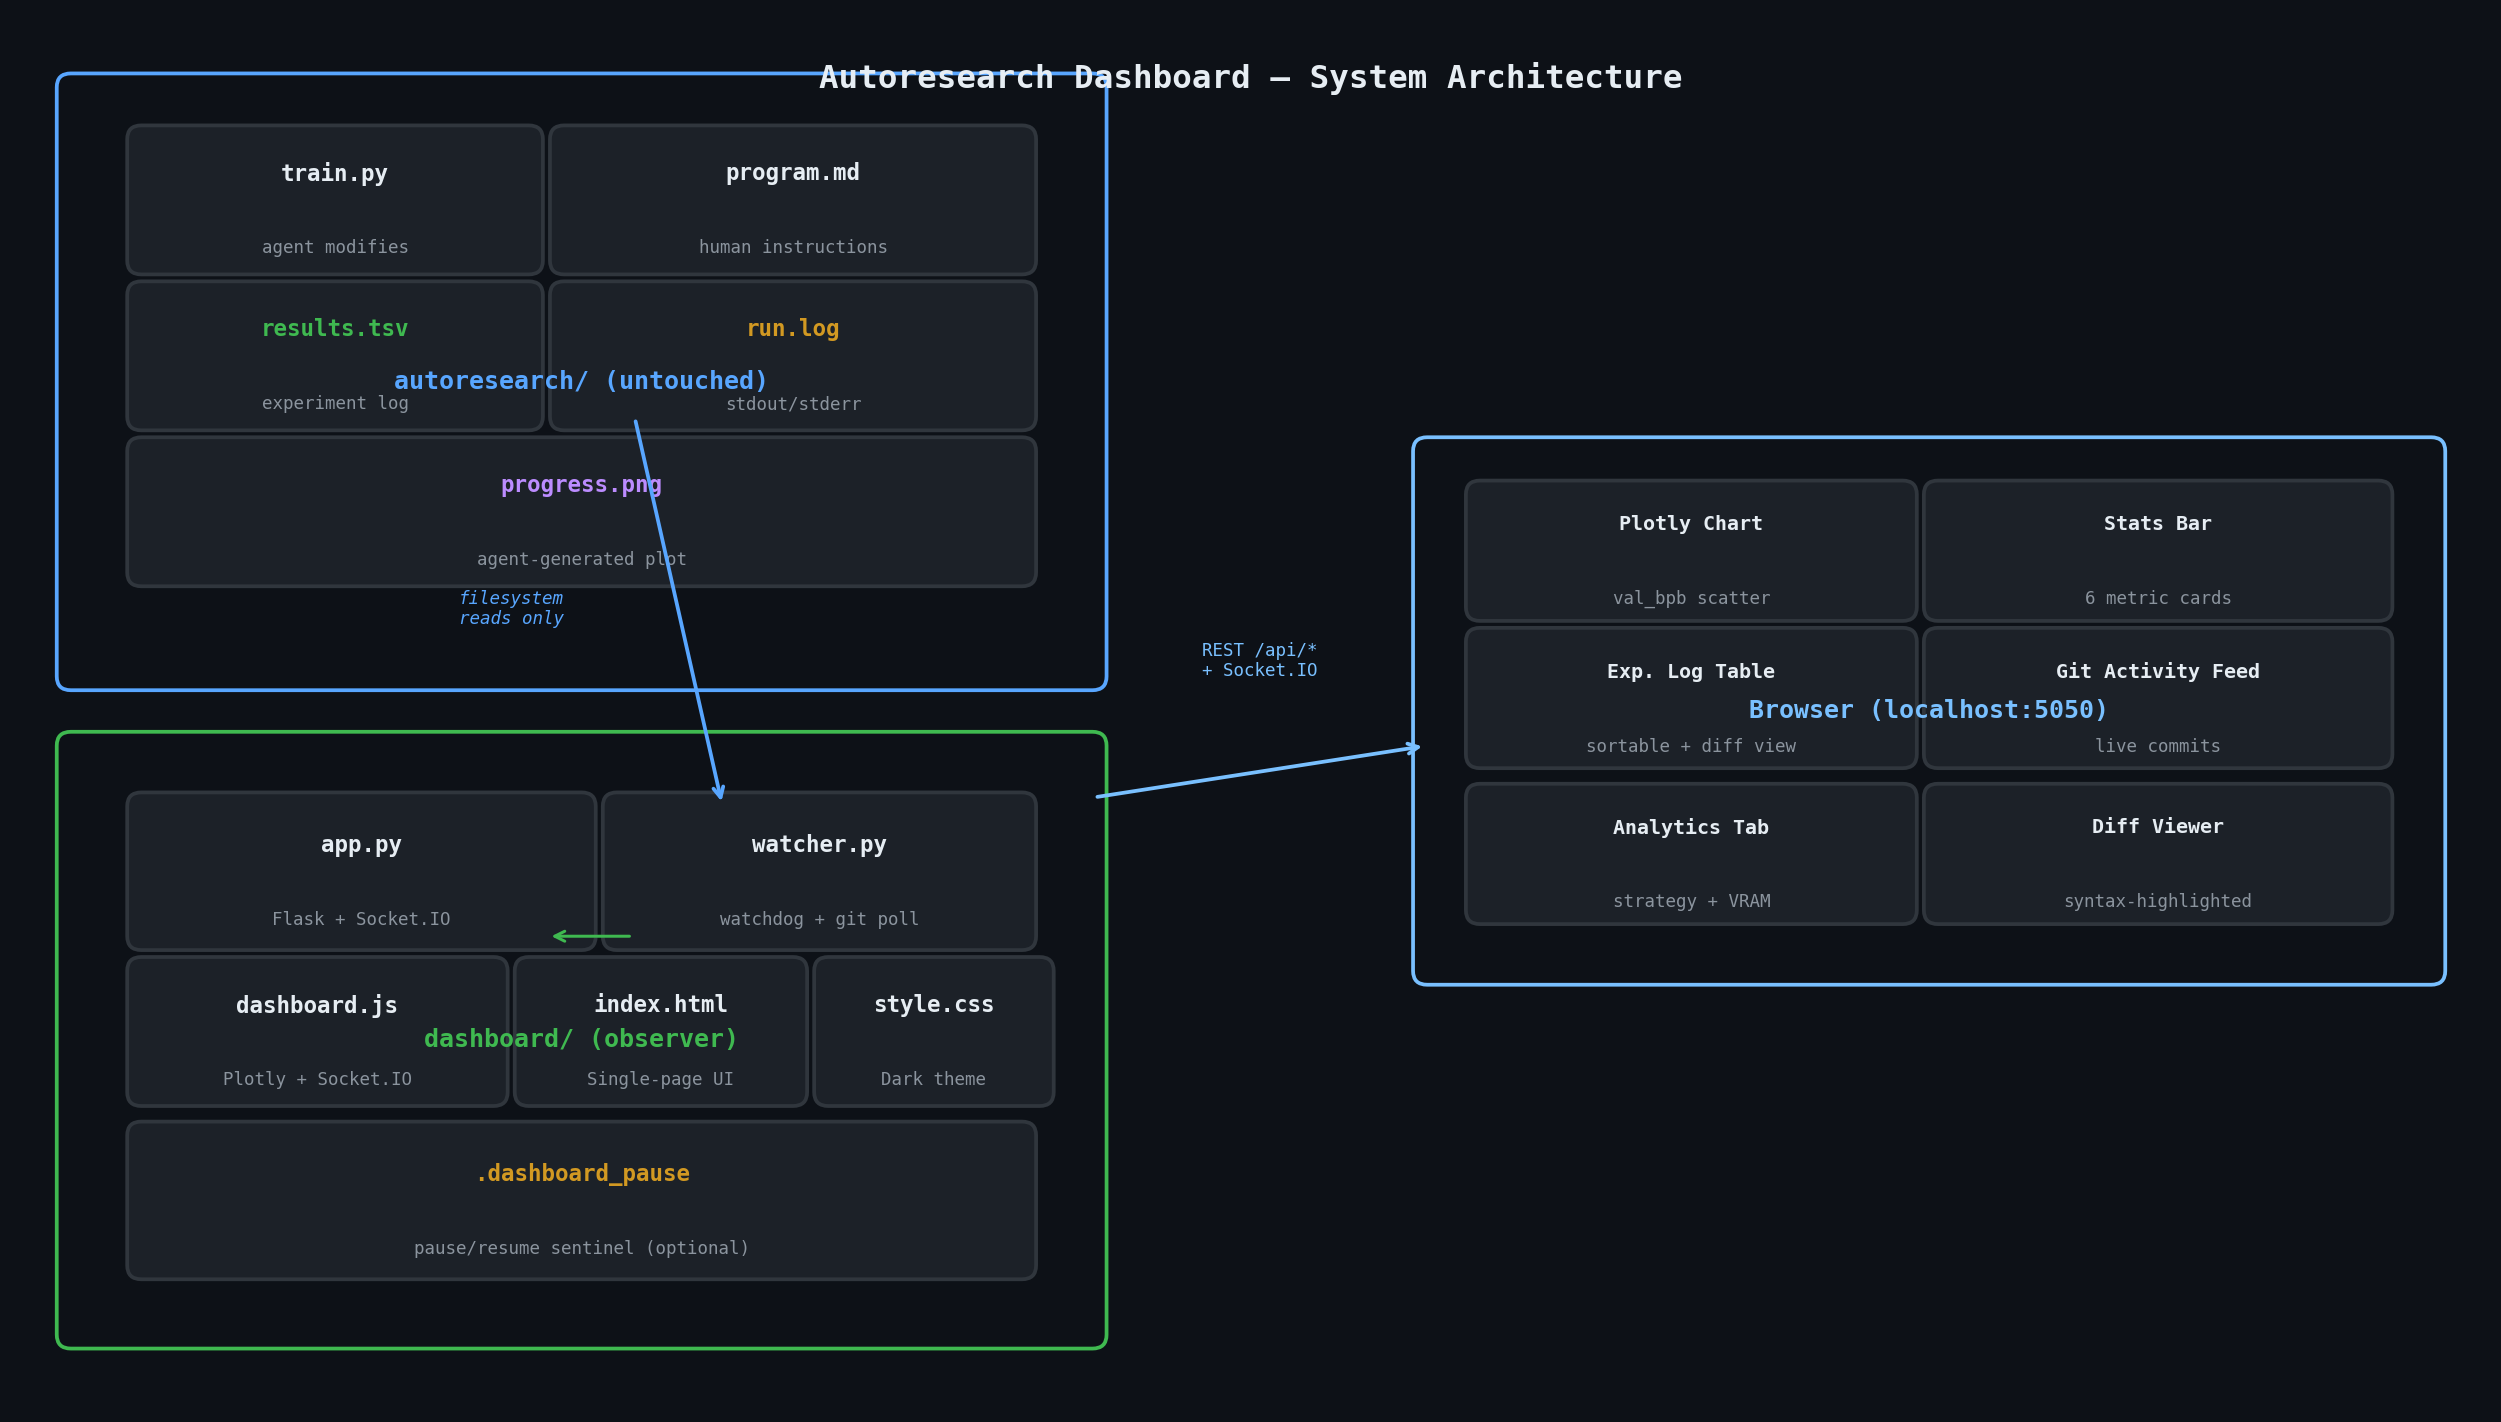
\includegraphics[width=0.92\textwidth]{figures/architecture.png}
  \vspace{2cm}

  {\large\color{text} Sanjana Singh\par}
  \vspace{0.3cm}
  {\normalsize\color{muted} \texttt{sanjana.singh@iitgn.ac.in}\par}
  \vspace{0.3cm}
  {\normalsize\color{muted} March 2026\par}
  \vspace{0.5cm}
  {\small\color{muted}
    Built on Karpathy's \href{https://github.com/karpathy/autoresearch}{autoresearch} ·
    Source: \href{https://github.com/sanjanasinghx/autoresearch-dashboard}{github.com/sanjanasinghx/autoresearch-dashboard}\par
  }
\end{titlepage}

% ── Table of Contents ────────────────────────────────────────────────────────
\tableofcontents
\newpage

% ─────────────────────────────────────────────────────────────────────────────
\section{Introduction}

Karpathy's \textit{autoresearch} is an autonomous ML experimentation loop in which a language model agent
repeatedly modifies \code{train.py}, runs 5-minute GPU training experiments, evaluates the model on a
held-out validation set (measuring \textit{val\_bpb}, validation bits-per-byte), and commits improvements
to a git branch. The agent is entirely self-directed: it reads the experiment log, forms hypotheses, applies
code changes, and iterates — with no human in the loop.

While the agent operates autonomously, practitioners still need to \textit{observe} the loop:
\begin{itemize}[leftmargin=1.5em]
  \item Is the agent making progress, or stuck in a no-gain plateau?
  \item Which architectural or optimiser changes have been tried?
  \item Is the GPU memory usage creeping up across experiments?
  \item Did the agent crash in the last run?
\end{itemize}

This report describes the \textbf{Autoresearch Dashboard} — a real-time web application that answers
these questions by passively observing the autoresearch repository's filesystem and git history, with
no modifications to the core agent loop.

\subsection{Design Constraint}

\begin{infobox}
\textbf{Key constraint:} the dashboard is a \emph{pure observer}. It never writes to
\code{train.py}, \code{prepare.py}, or \code{program.md}. The only optional touch-point is a
\code{.dashboard\_pause} sentinel file the user can have the agent check before each experiment.
\end{infobox}

% ─────────────────────────────────────────────────────────────────────────────
\section{System Architecture}

\subsection{Overview}

\begin{figure}[h]
  \centering
  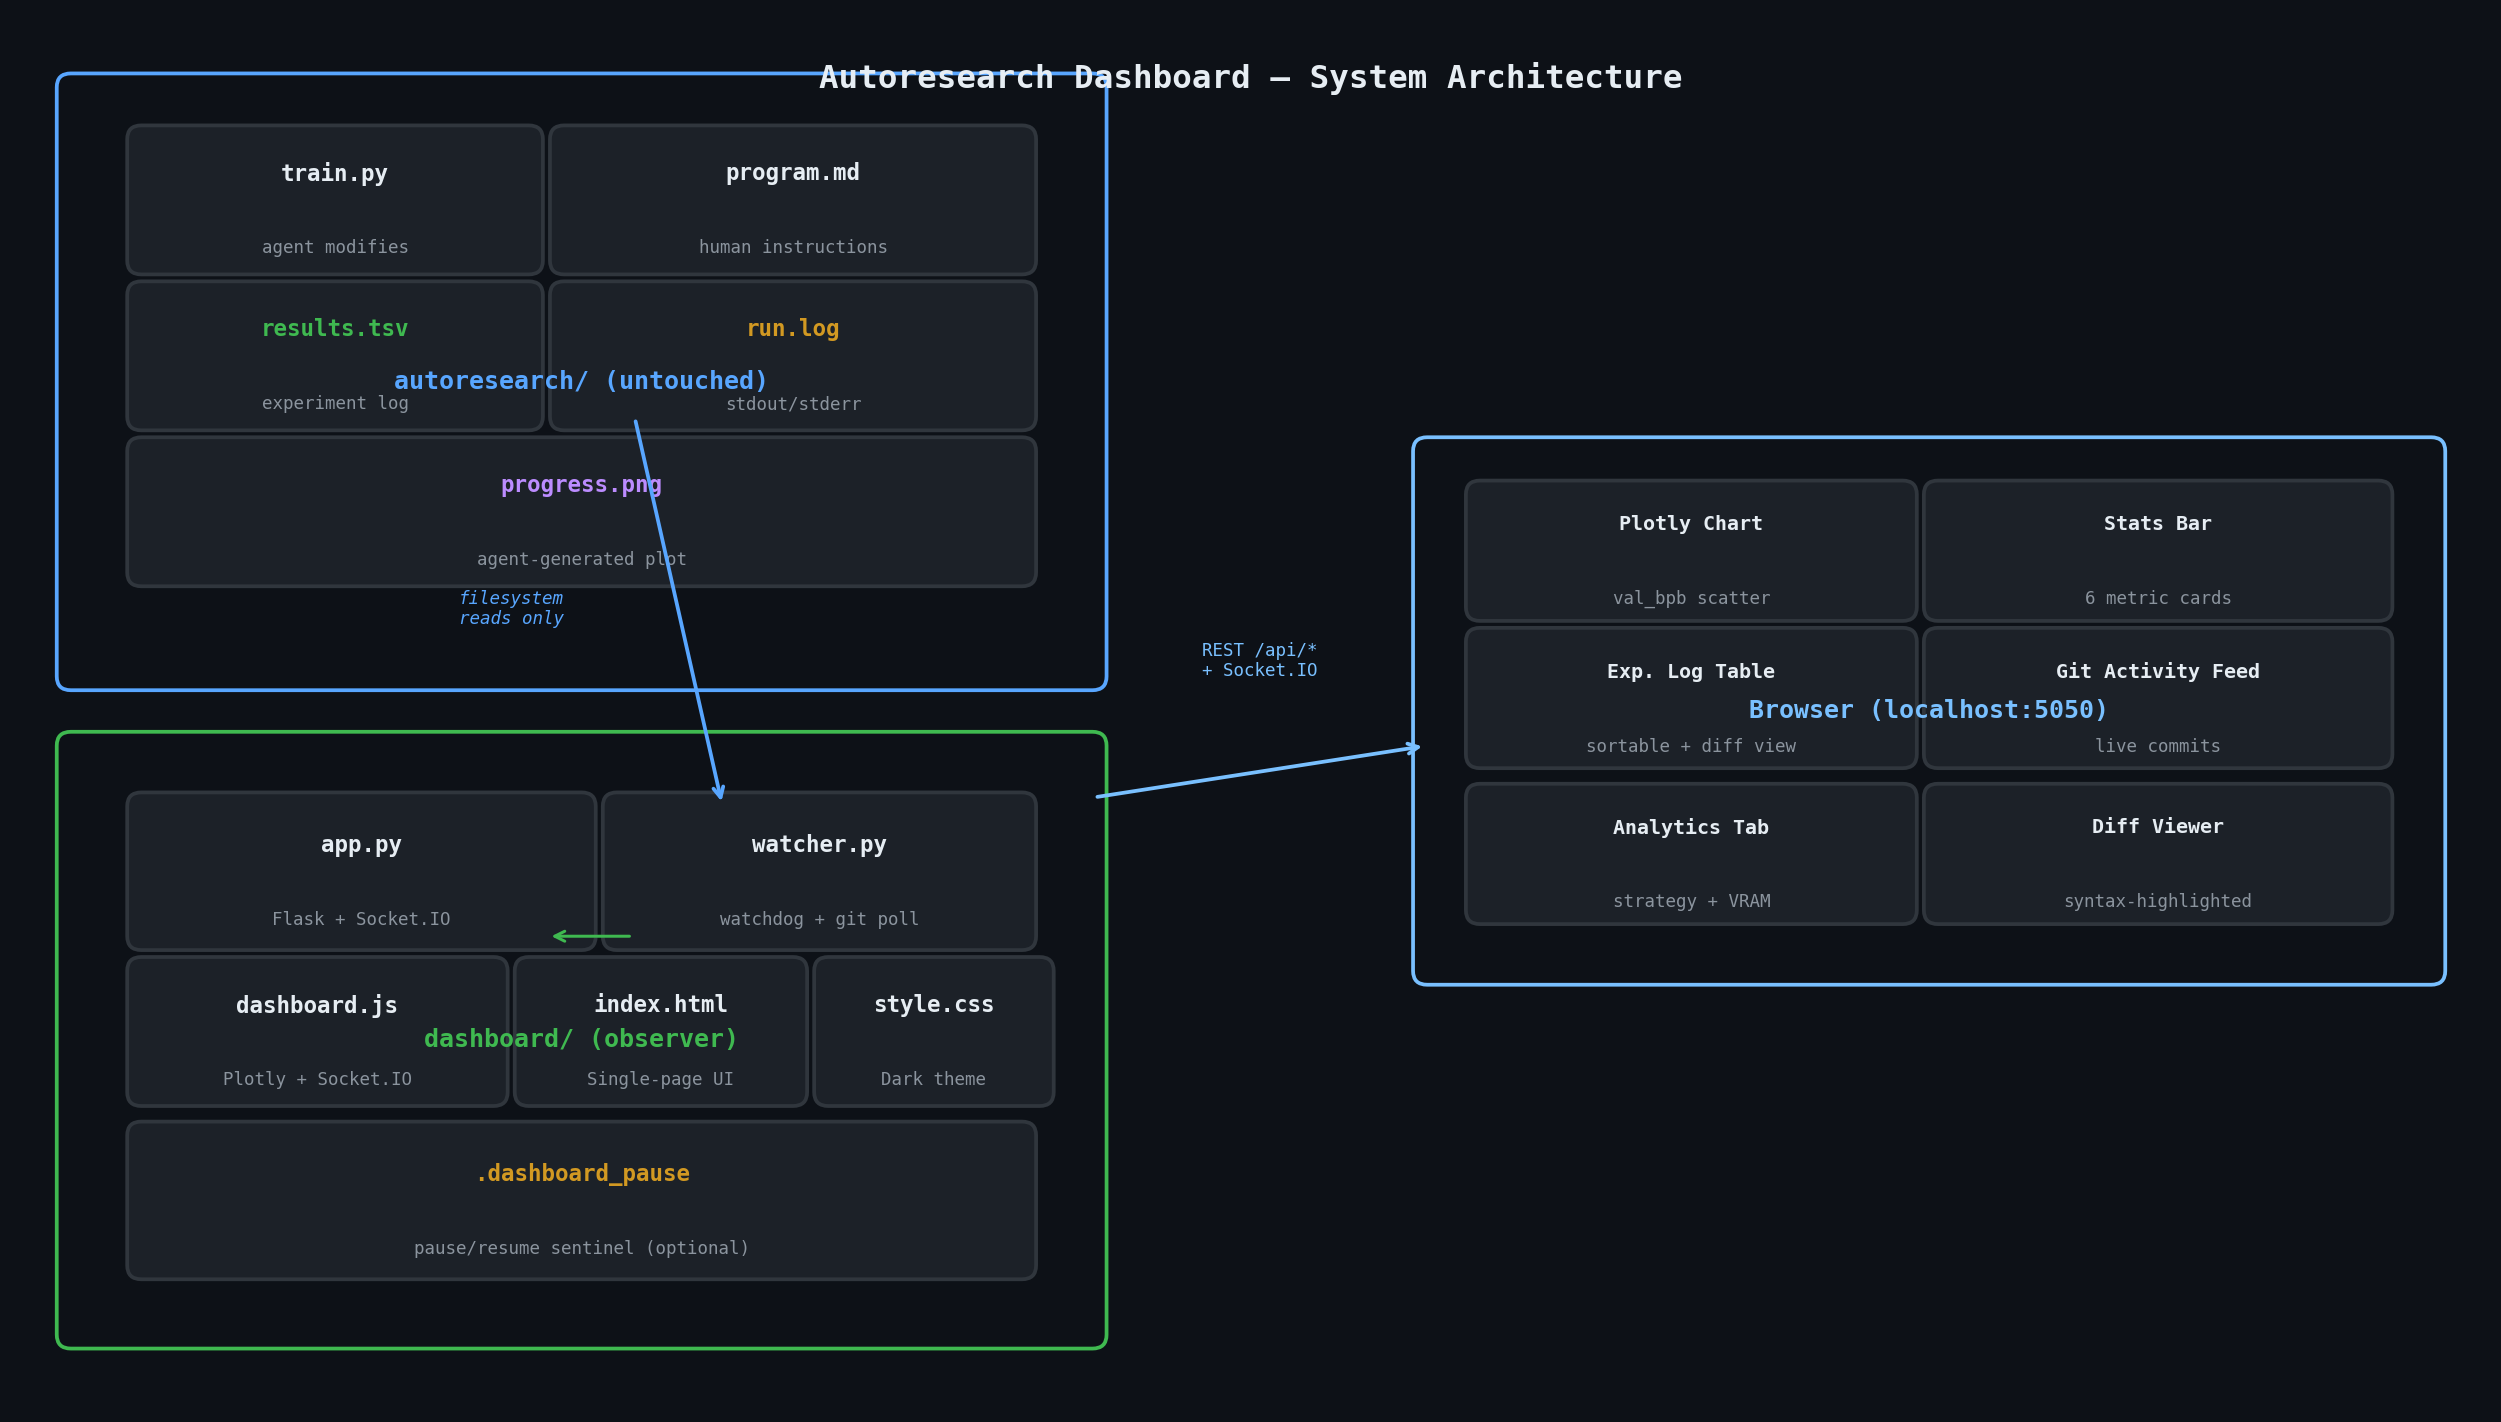
\includegraphics[width=\textwidth]{figures/architecture.png}
  \caption{System architecture. The dashboard (green box) reads filesystem state and git history from
           the autoresearch repo (blue box) and serves a single-page web application to the browser
           (cyan box) via REST and Socket.IO.}
  \label{fig:arch}
\end{figure}

The system is composed of three layers (Figure~\ref{fig:arch}):

\begin{description}[leftmargin=1.5em, style=nextline]
  \item[\textcolor{blue}{Autoresearch repo (untouched)}]
    The agent's working directory containing \code{train.py} (modified each experiment),
    \code{results.tsv} (one row per completed experiment), \code{run.log} (live stdout/stderr),
    and \code{progress.png} (agent-generated plot).
  \item[\textcolor{green}{dashboard/ (observer)}]
    A Flask + Socket.IO Python server with a background watcher daemon. Reads filesystem state
    and git history; emits WebSocket events to connected browsers.
  \item[\textcolor{purple}{Browser}]
    A single-page application built with Plotly.js and the Socket.IO client (both from CDN, no
    build step). Updates in real time as experiments complete.
\end{description}

\subsection{File Structure}

\begin{lstlisting}[language=bash, caption={Dashboard file structure}]
autoresearch/
├── train.py          # agent modifies (UNTOUCHED by dashboard)
├── prepare.py        # fixed evaluation code (UNTOUCHED)
├── program.md        # human instructions (UNTOUCHED)
├── results.tsv       # parsed by dashboard
├── run.log           # tailed by dashboard
├── progress.png      # served by dashboard
└── dashboard/
    ├── app.py              # Flask + Socket.IO server
    ├── watcher.py          # Filesystem + git monitoring
    ├── run_mock_agent.py   # Simulation script for testing
    ├── requirements.txt
    ├── Dockerfile
    ├── static/
    │   ├── dashboard.js    # Plotly + Socket.IO client
    │   └── dashboard.css   # Dark theme (JetBrains Mono)
    └── templates/
        └── index.html      # Single-page layout
\end{lstlisting}

% ─────────────────────────────────────────────────────────────────────────────
\section{Backend Implementation}

\subsection{Results TSV Parser (\texttt{watcher.py})}

The \code{parse\_results()} function reads the agent's \code{results.tsv} with columns
\code{experiment\_id}, \code{val\_bpb}, \code{peak\_vram\_mb}, \code{commit\_sha},
\code{timestamp}, and \code{description}. It computes three derived columns:

\begin{lstlisting}[language=Python, caption={Derived column computation in parse\_results()}]
df["cumulative_best"] = df["val_bpb"].expanding().min()
prev_best = df["cumulative_best"].shift(1)
df["delta_bpb"] = df["val_bpb"] - prev_best

def classify(row):
    if pd.isna(row["val_bpb"]):  return "crashed"
    if row["delta_bpb"] < -1e-6: return "improved"
    return "no_gain"

df["status"] = df.apply(classify, axis=1)
\end{lstlisting}

The \code{parse\_run\_log()} function greps the live \code{run.log} for the last
\code{val\_bpb} and \code{peak\_vram\_mb} values, detects Python tracebacks to identify crashes,
and returns the last 20 lines as a tail for the live log panel.

\subsection{Git Tracker (\texttt{watcher.py})}

The \code{GitTracker} class wraps GitPython to enumerate \code{autoresearch/*} branches,
extract commit history with accurate diff statistics (insertions/deletions via
\code{commit.stats}), and parse \code{val\_bpb} values embedded in commit messages:

\begin{lstlisting}[language=Python, caption={Extracting val\_bpb from commit messages}]
m = re.search(r"val_bpb[:\s=]+([0-9]+\.[0-9]+)", commit.message)
if m:
    val_bpb = float(m.group(1))
\end{lstlisting}

\subsection{Filesystem Watcher (\texttt{watcher.py})}

\code{ExperimentWatcher} uses the \texttt{watchdog} library for immediate filesystem events,
backed by a 10-second fallback polling loop for robustness. Critically, it initialises
\code{last\_experiment\_count} to the \textit{current} row count on startup — preventing all
existing experiments from re-broadcasting as ``new'' events when the server restarts.

\begin{lstlisting}[language=Python, caption={Initialise count to avoid re-broadcasting old experiments}]
class ExperimentWatcher:
    def __init__(self, repo_path, socketio):
        ...
        # Initialise to current count so old experiments don't re-emit
        tsv_path = os.path.join(repo_path, "results.tsv")
        self.last_experiment_count = len(parse_results(tsv_path))
\end{lstlisting}

\subsection{Flask API Endpoints (\texttt{app.py})}

\begin{figure}[h]
  \centering
  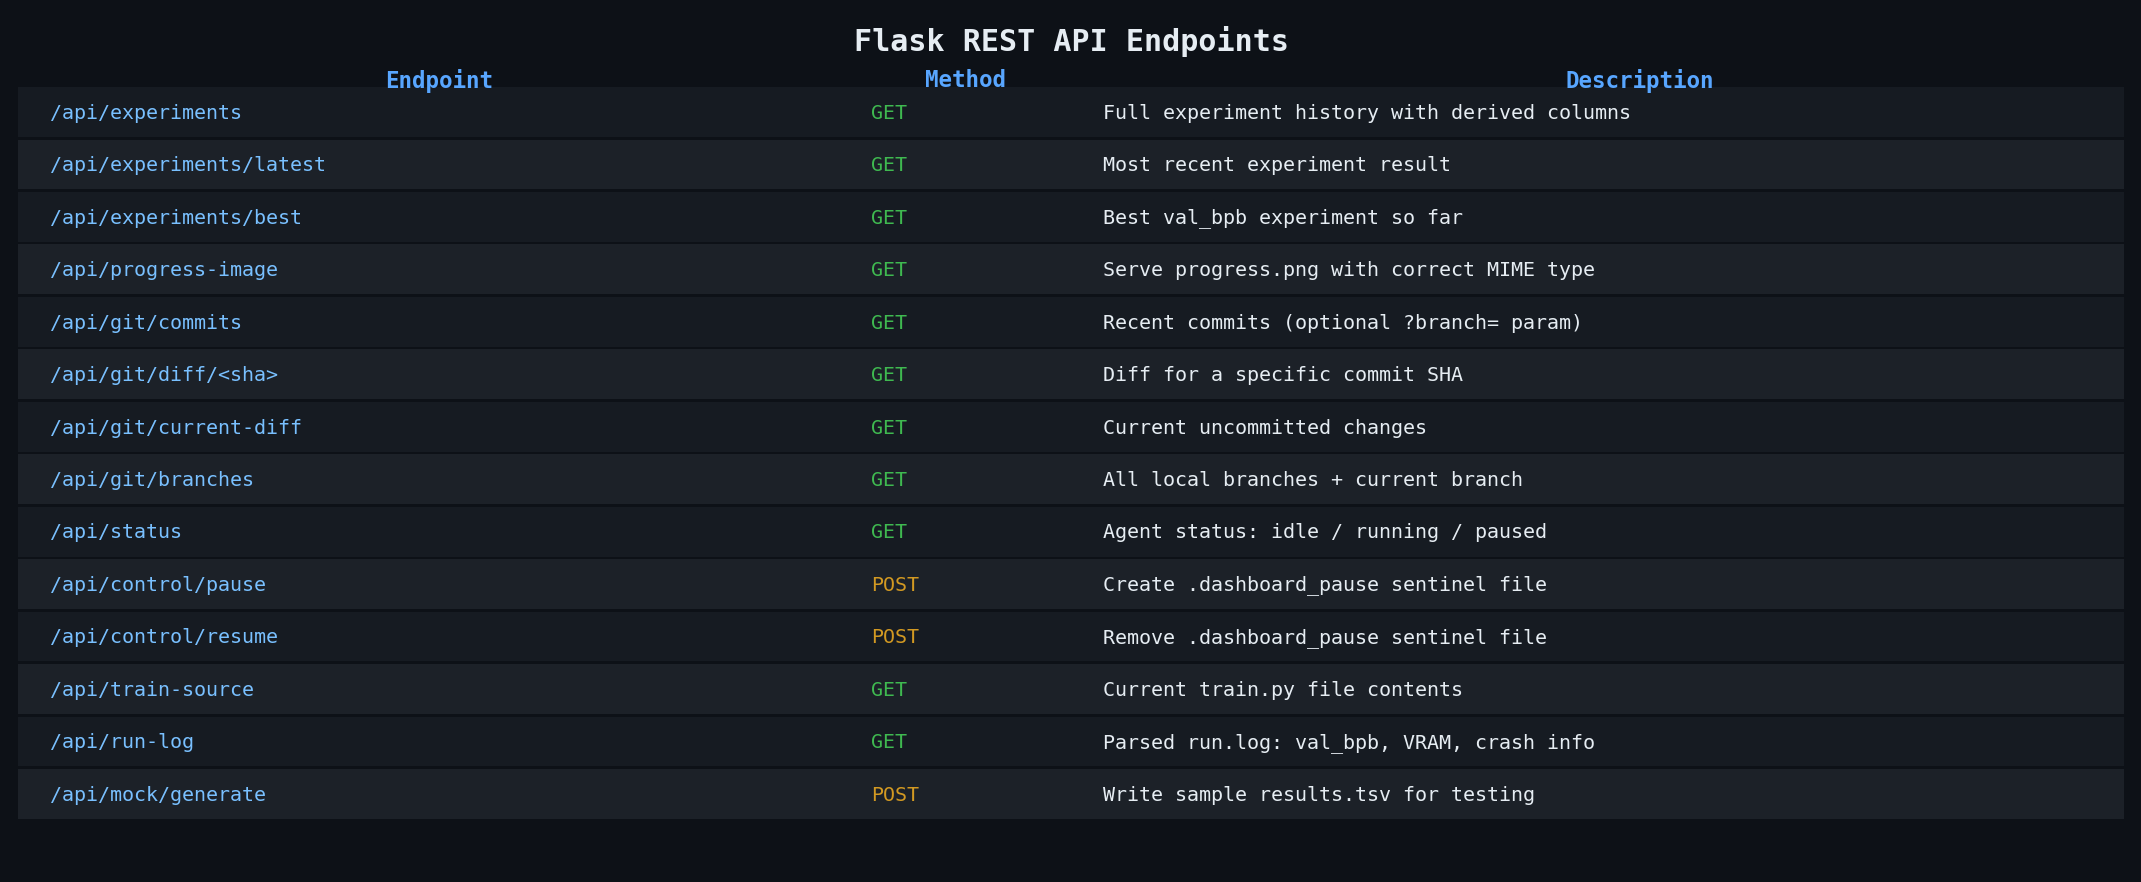
\includegraphics[width=\textwidth]{figures/api_table.png}
  \caption{All 14 REST API endpoints exposed by the Flask server. GET endpoints are read-only;
           the two POST endpoints (pause/resume) only create or delete a sentinel file.}
  \label{fig:api}
\end{figure}

A key bug discovered during development: using \code{socketio.emit(\ldots, to=sid)} inside a
Flask-SocketIO event handler silently does nothing (it is the broadcast API, not the per-client
API). The correct call is \code{emit()} imported from \code{flask\_socketio}, which automatically
targets the requesting client:

\begin{lstlisting}[language=Python, caption={Correct Socket.IO emit inside a handler}]
from flask_socketio import SocketIO, emit as ws_emit

@socketio.on("connect")
def on_connect():
    ws_emit("full_state", {"experiments": records})  # correct
    # socketio.emit(..., to=request.sid)             # WRONG - silent no-op
\end{lstlisting}

\subsection{Real-Time Event Flow}

\begin{figure}[h]
  \centering
  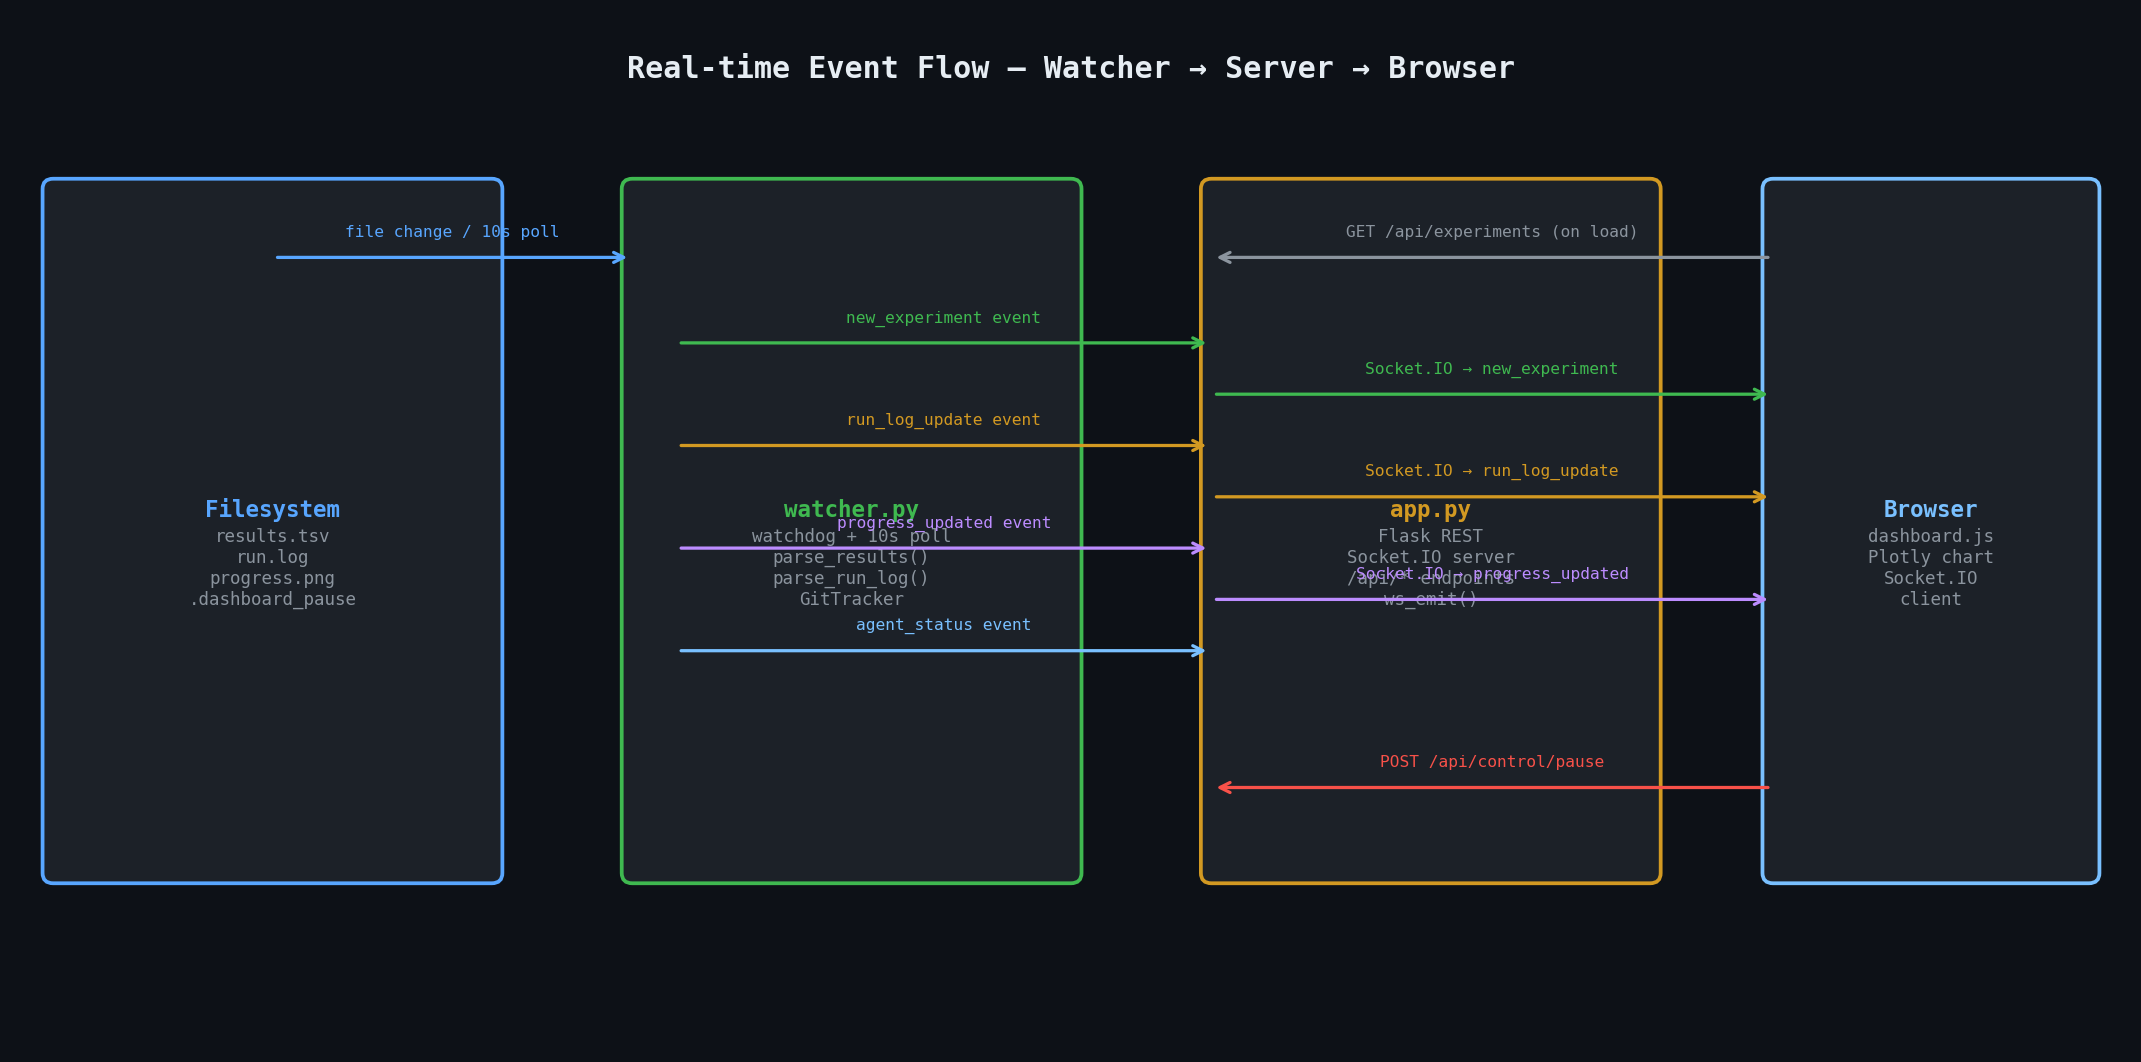
\includegraphics[width=\textwidth]{figures/event_flow.png}
  \caption{Socket.IO event flow from filesystem change through watcher, server, and into the
           browser. REST calls (grey/red arrows) provide the initial page load state and control actions.}
  \label{fig:events}
\end{figure}

Table~\ref{tab:events} lists the Socket.IO events emitted by the watcher.

\begin{table}[h]
\centering
\caption{Socket.IO events and their frontend actions}
\label{tab:events}
\begin{tabular}{@{}lll@{}}
\toprule
\textbf{Event} & \textbf{Payload} & \textbf{Frontend Action} \\
\midrule
\code{new\_experiment}   & \code{\{experiment\_number, val\_bpb, status, \ldots\}} & Add dot to chart, prepend table row, update stats \\
\code{new\_commit}       & \code{\{sha, message, timestamp, diff\_stat\}}          & Prepend to git activity feed \\
\code{progress\_updated} & \code{\{timestamp\}}                                    & Reload \code{progress.png} image \\
\code{run\_log\_update}  & \code{\{tail: [...lines], crashed: bool\}}              & Update live log footer \\
\code{agent\_status}     & \code{\{status: "running"|"paused"|"idle"\}}            & Update status indicator \\
\code{full\_state}       & \code{\{experiments: [...]\}}                           & Initialise chart and table on connect \\
\bottomrule
\end{tabular}
\end{table}

% ─────────────────────────────────────────────────────────────────────────────
\section{Frontend Implementation}

\subsection{Dashboard Layout}

The single-page dashboard is structured into five areas:

\begin{enumerate}[leftmargin=1.5em]
  \item \textbf{Header bar} — branch selector, status indicator (pulsing green dot when running),
        ETA to next run, and pause/resume button.
  \item \textbf{Stats bar} — six metric cards: total experiments, best val\_bpb, improvement rate,
        crash count, average $\Delta$bpb, and total runtime.
  \item \textbf{Main chart} — interactive Plotly scatter plot (Section~\ref{sec:chart}).
  \item \textbf{Tabbed panel} — Experiment Log, Analytics, and Diff Viewer tabs.
  \item \textbf{Right sidebar} — \code{progress.png} viewer, git activity feed, live run.log tail.
\end{enumerate}

\subsection{Progress Chart}
\label{sec:chart}

\begin{figure}[h]
  \centering
  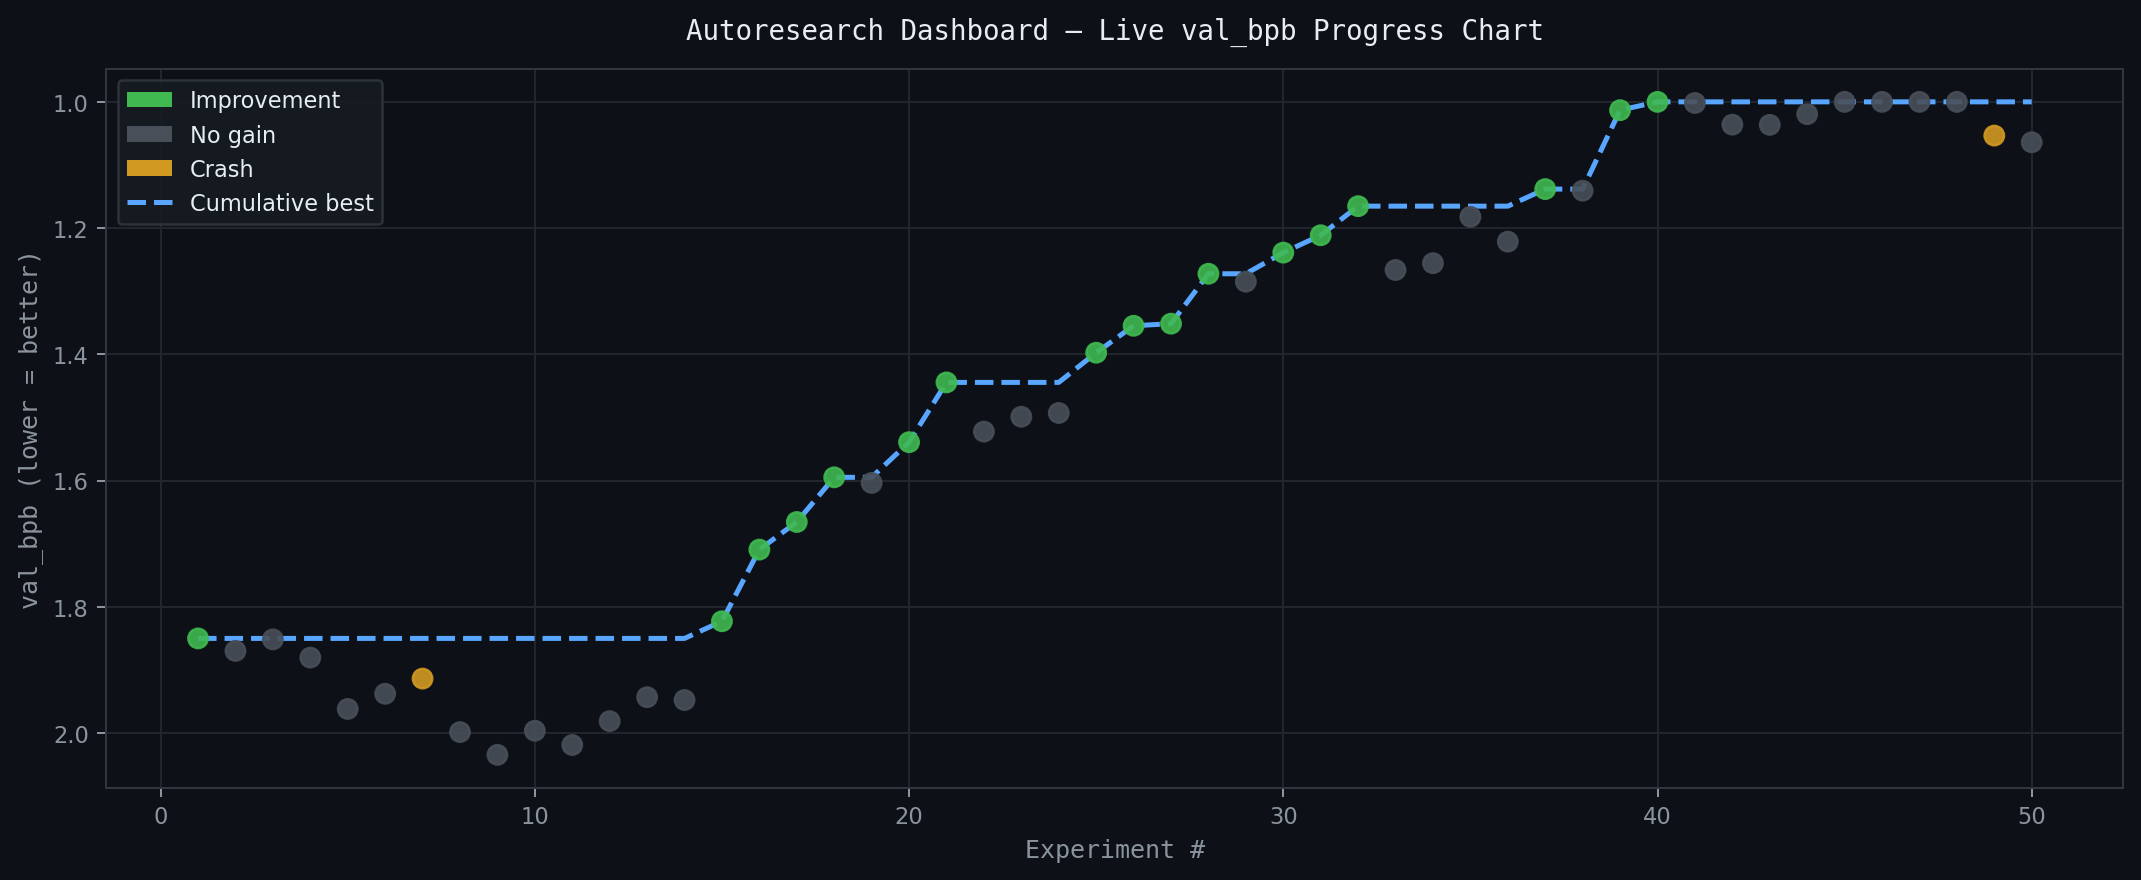
\includegraphics[width=\textwidth]{figures/progress_chart.png}
  \caption{The interactive Plotly val\_bpb scatter chart. Green dots indicate experiments that
           improved the best-so-far score; grey dots are no-gain; orange markers are crashes.
           The dashed blue line tracks the cumulative minimum (best val\_bpb achieved).
           Y-axis is inverted since lower val\_bpb is better.}
  \label{fig:chart}
\end{figure}

The chart is built with Plotly.js in \code{scatter} mode. Two traces are rendered per branch:
a dot-per-experiment scatter trace with per-dot colour coding, and a dashed line trace showing
the running minimum \code{cumulative\_best}. When multiple branches are selected in overlay mode,
each branch receives a distinct colour from the palette.

The chart uses \textit{lazy initialisation} — if the Plotly CDN has not loaded by the time
\code{window.load} fires, it degrades gracefully (showing a message) without blocking the
experiment table from rendering.

\subsection{CDN Loading Bug Fix}

A subtle frontend bug: the original code placed Plotly and Socket.IO \code{<script>} tags in
\code{<head>}, used \code{DOMContentLoaded} as the boot trigger, and called \code{initChart()}
without a try/catch. On a slow CDN connection:

\begin{enumerate}[leftmargin=1.5em]
  \item \code{DOMContentLoaded} fires before CDN scripts finish loading
  \item \code{Plotly} is undefined → \code{Plotly.newPlot()} throws
  \item The exception propagates and \code{renderAll()} never runs
  \item Table stays empty; stats stay as dashes
\end{enumerate}

The fix moves CDN scripts to end of \code{<body>}, switches the boot trigger to
\code{window.load} (guaranteed to fire after all scripts), and wraps chart init in try/catch
so table rendering is independent of chart availability.

\subsection{Analytics Panel}

\begin{figure}[h]
  \centering
  \begin{subfigure}[b]{0.52\textwidth}
    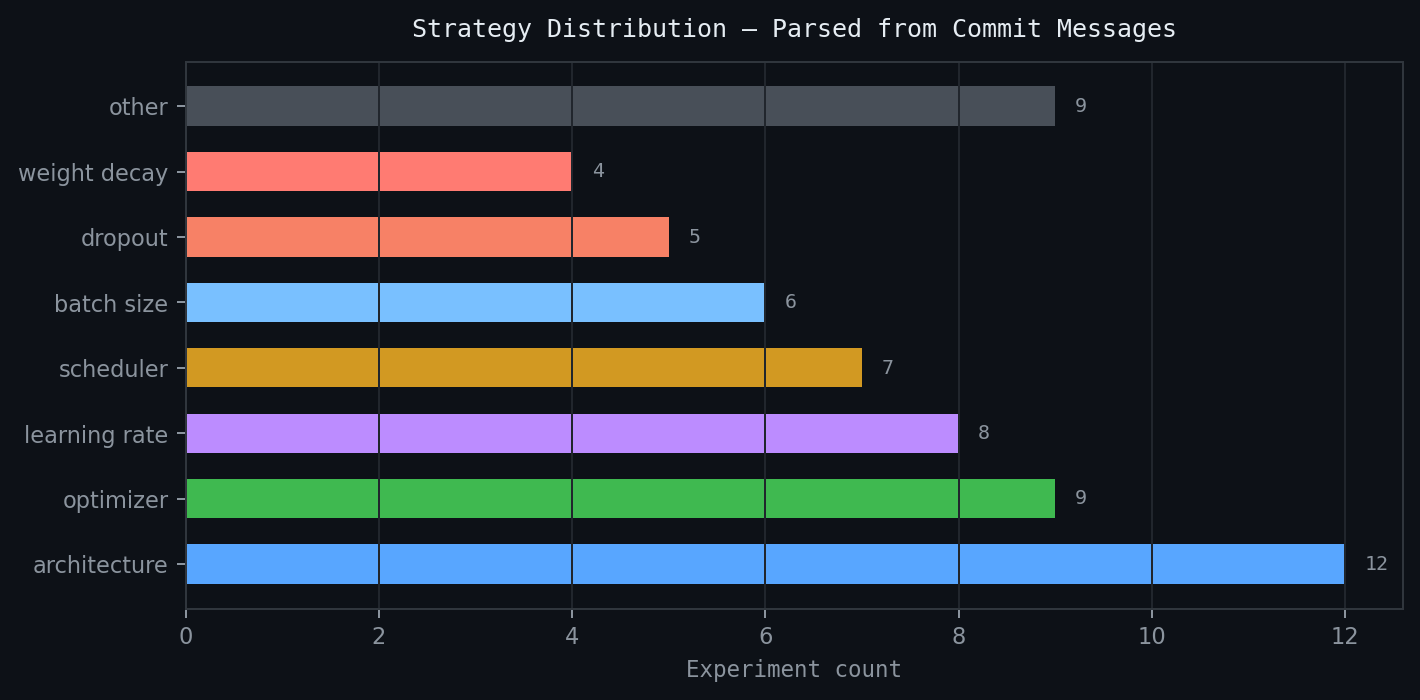
\includegraphics[width=\textwidth]{figures/strategy_dist.png}
    \caption{Strategy distribution: experiment descriptions are parsed by keyword matching to
             categorise the agent's exploration strategy.}
    \label{fig:strategy}
  \end{subfigure}
  \hfill
  \begin{subfigure}[b]{0.46\textwidth}
    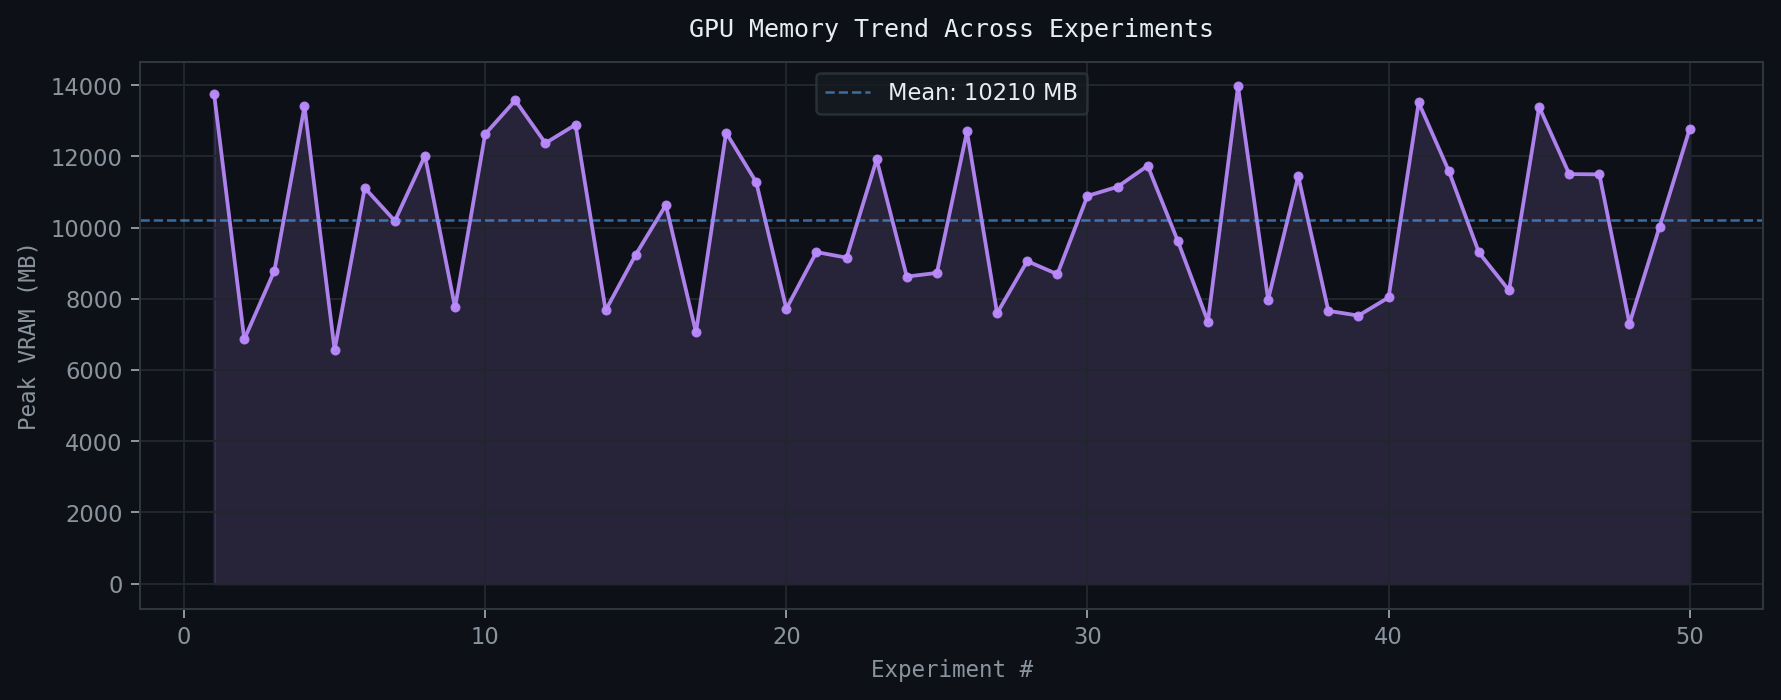
\includegraphics[width=\textwidth]{figures/vram_trend.png}
    \caption{GPU memory trend across experiments. Dashed blue line shows the mean VRAM usage;
             filled area visualises variance.}
    \label{fig:vram}
  \end{subfigure}
  \caption{Analytics tab charts.}
\end{figure}

The analytics tab computes four key insights:
\begin{itemize}[leftmargin=1.5em]
  \item \textbf{Experiments per hour} — derived from the timestamp range of \code{results.tsv}
  \item \textbf{Time since last improvement} — index of the last row with \code{status = "improved"}
  \item \textbf{Longest no-gain streak} — computed in a single pass over the status column
  \item \textbf{Average VRAM} — mean of non-null \code{peak\_vram\_mb} values
\end{itemize}

% ─────────────────────────────────────────────────────────────────────────────
\section{Pause / Resume Mechanism}

The pause/resume feature is entirely non-invasive. The dashboard's \textbf{Pause} button sends
a \code{POST /api/control/pause} request, which creates a \code{.dashboard\_pause} file in the
repo root. The \textbf{Resume} button deletes it.

To honour this signal, users can optionally add a single line to \code{program.md}:

\begin{infobox}
\texttt{Before starting each new experiment, check if a file \textbf{.dashboard\_pause} exists
in the repo root. If it does, wait and check again every 30 seconds until it is removed.}
\end{infobox}

This is the \textit{only} optional modification to the autoresearch workflow, and it is
entirely at the user's discretion.

% ─────────────────────────────────────────────────────────────────────────────
\section{Karpathy's progress.png}

\begin{figure}[h]
  \centering
  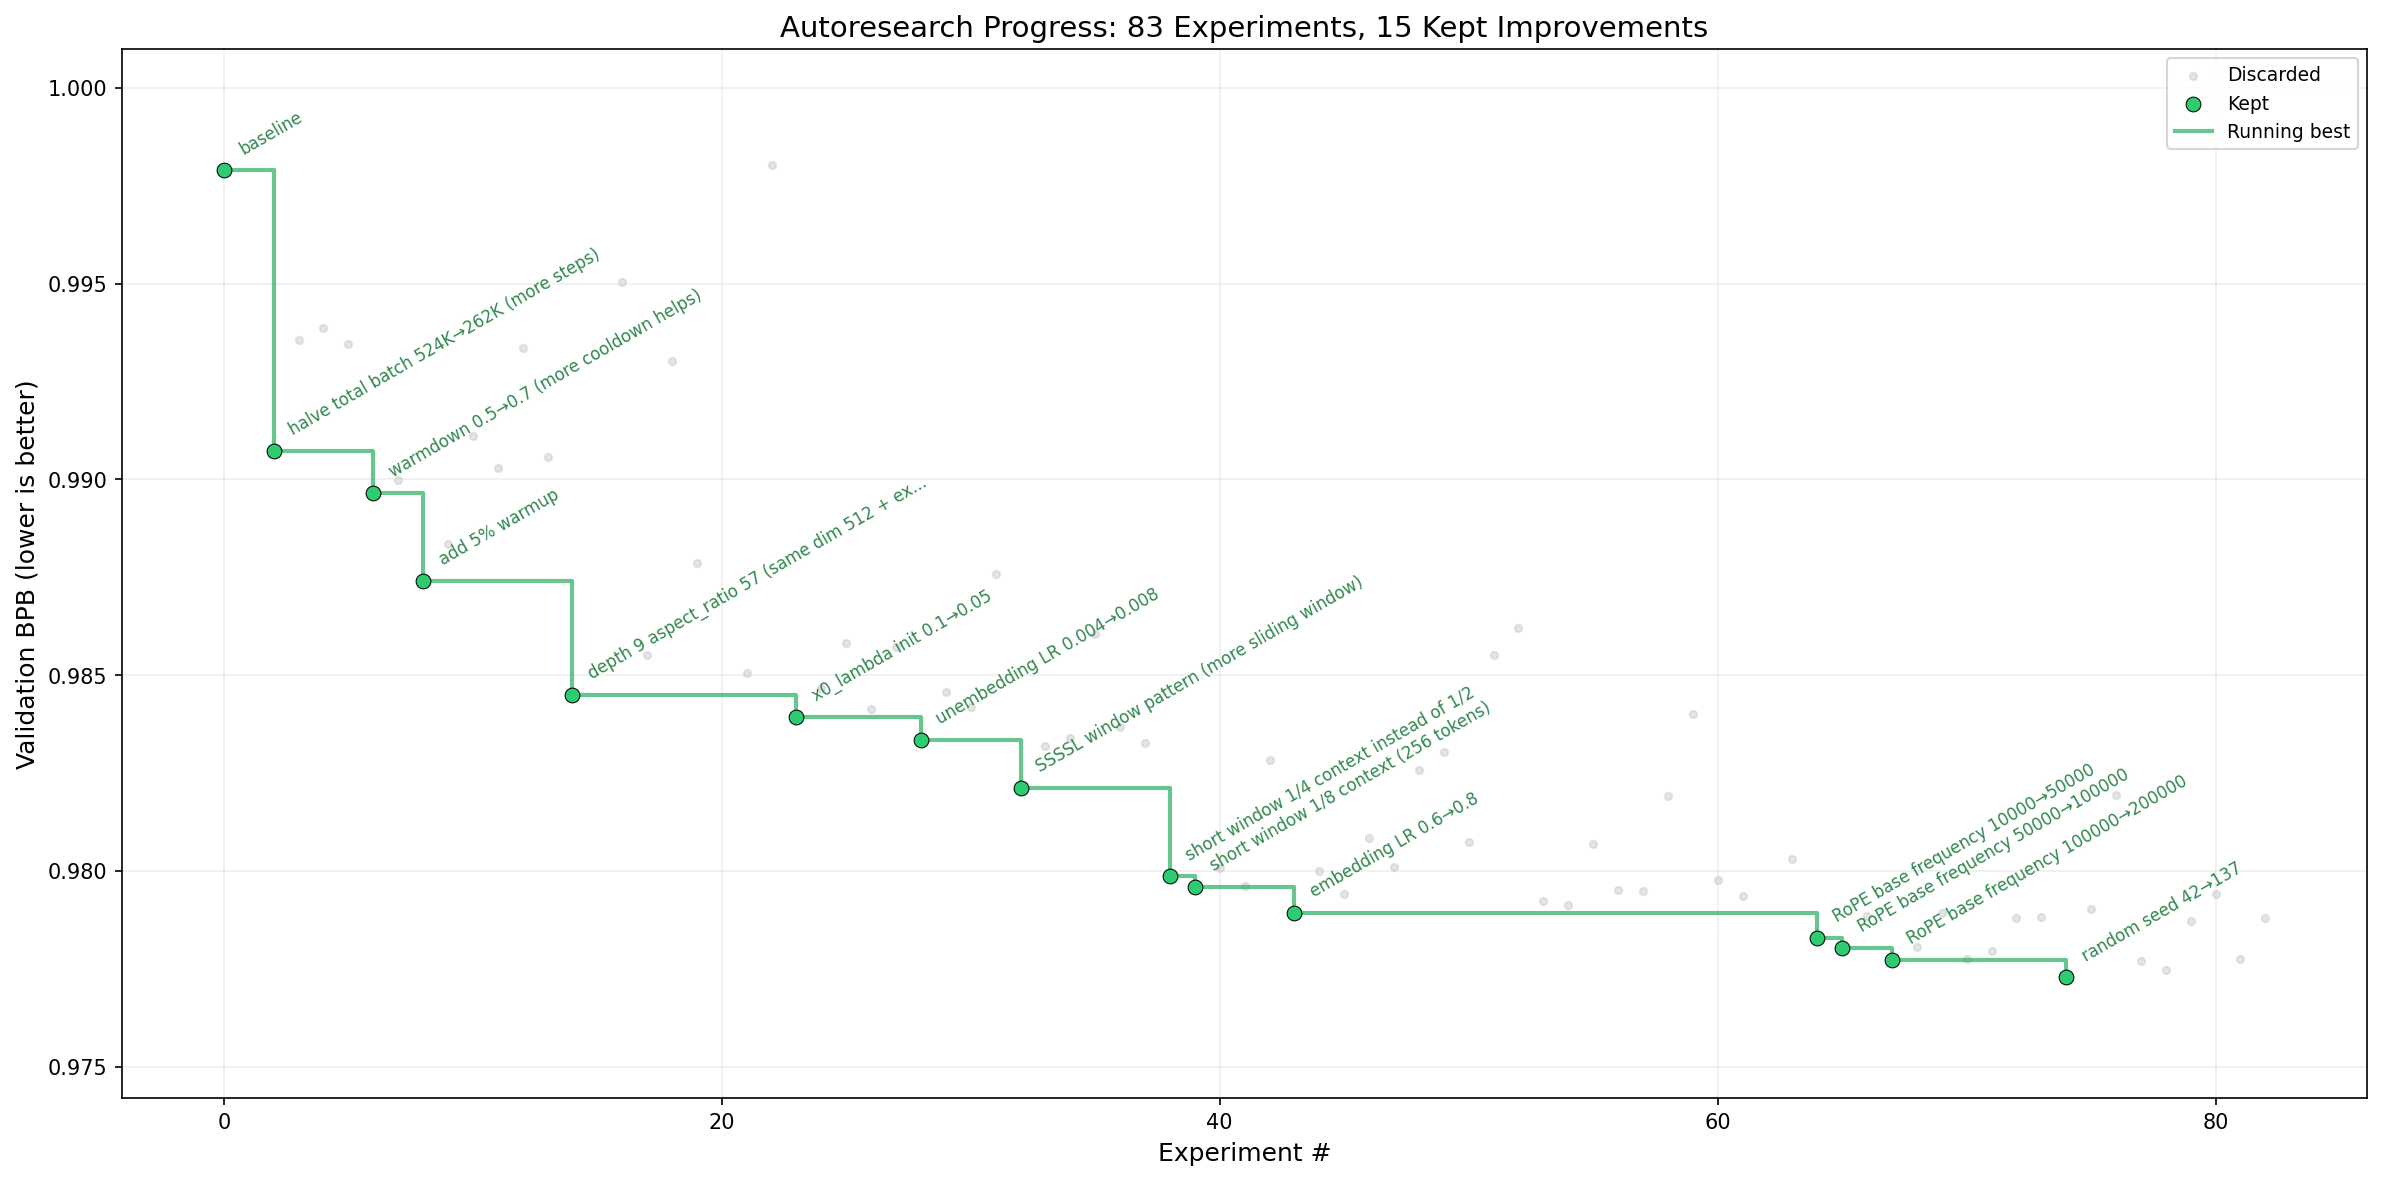
\includegraphics[width=0.85\textwidth]{figures/progress.png}
  \caption{The \texttt{progress.png} generated by the autoresearch agent itself, served
           directly from the filesystem at \code{/api/progress-image} and auto-refreshed in the
           dashboard's right sidebar whenever the file changes.}
  \label{fig:progress}
\end{figure}

The dashboard's right sidebar embeds the agent's own \code{progress.png} (Figure~\ref{fig:progress}),
auto-refreshing it whenever the \code{progress\_updated} Socket.IO event fires (triggered by the
watcher detecting a file modification). This gives a secondary view consistent with the agent's
own visualisation, complementing the dashboard's interactive Plotly chart.

% ─────────────────────────────────────────────────────────────────────────────
\section{Multi-Branch Support}

When multiple \code{autoresearch/*} branches exist in the repository (e.g., from different
experimental sessions or different \code{program.md} prompts), the branch selector in the
dashboard header lets users switch between them. Enabling \textbf{Overlay mode} plots all branches
on the same chart in distinct colours, with a legend, enabling direct comparison of exploration
trajectories.

A branch comparison table (in the Analytics tab) shows each branch's best val\_bpb, total
experiment count, and improvement rate side-by-side.

% ─────────────────────────────────────────────────────────────────────────────
\section{Testing and Mock Agent}

The \code{run\_mock\_agent.py} script simulates the autoresearch loop for testing the dashboard
without a GPU:

\begin{lstlisting}[language=bash, caption={Running the mock agent}]
python dashboard/run_mock_agent.py \
    --repo /path/to/autoresearch \
    --interval 5 \   # seconds between experiments
    --count 50        # total experiments to simulate
\end{lstlisting}

The mock agent:
\begin{itemize}[leftmargin=1.5em]
  \item Appends one row to \code{results.tsv} per interval with realistic val\_bpb drift
  \item Simulates an 8\% crash rate (rows with missing val\_bpb)
  \item Writes intermediate progress to \code{run.log} mid-experiment
  \item Checks for the \code{.dashboard\_pause} sentinel and blocks until removed
\end{itemize}

A separate \code{POST /api/mock/generate} endpoint writes a 20-row sample \code{results.tsv}
instantly for UI exploration without running the agent.

% ─────────────────────────────────────────────────────────────────────────────
\section{Deployment}

\subsection{Local}

\begin{lstlisting}[language=bash, caption={Local setup and launch}]
cd autoresearch
pip install -r dashboard/requirements.txt
python dashboard/app.py --repo . --port 5050
# Open http://localhost:5050
\end{lstlisting}

\subsection{Docker}

\begin{lstlisting}[language=Dockerfile, caption={Dockerfile}]
FROM python:3.12-slim
WORKDIR /app
COPY dashboard/ .
RUN pip install --no-cache-dir -r requirements.txt
EXPOSE 5050
ENV AUTORESEARCH_REPO=/repo
CMD ["python", "app.py", "--repo", "/repo", "--port", "5050"]
\end{lstlisting}

\begin{lstlisting}[language=bash, caption={Docker run with volume mount}]
docker build -t autoresearch-dashboard ./dashboard
docker run -p 5050:5050 \
    -v /path/to/autoresearch:/repo \
    autoresearch-dashboard
\end{lstlisting}

% ─────────────────────────────────────────────────────────────────────────────
\section{Key Bugs Encountered and Fixed}

\begin{table}[h]
\centering
\caption{Bugs encountered during development and their root causes}
\label{tab:bugs}
\begin{tabular}{@{}p{3.2cm}p{5.5cm}p{5.5cm}@{}}
\toprule
\textbf{Symptom} & \textbf{Root Cause} & \textbf{Fix} \\
\midrule
Table shows ``No experiments yet'' despite data existing &
\code{socketio.emit(\ldots, to=sid)} inside a socket handler is a silent no-op;
\code{full\_state} never reached the browser &
Use \code{emit()} from \code{flask\_socketio} inside socket handlers \\
\addlinespace
Chart empty, stats show dashes &
\code{initChart()} called without try/catch; CDN failure throws → \code{renderAll()} never runs &
Wrap chart init in try/catch; boot on \code{window.load}; CDN scripts at end of \code{<body>} \\
\addlinespace
All existing experiments re-emit as ``new'' on server restart &
\code{last\_experiment\_count} initialised to 0, not current count &
Read \code{results.tsv} on watcher init and set count accordingly \\
\addlinespace
Inaccurate diff +/- line counts &
Manually counting \code{+}/\code{-} lines from raw patch bytes includes header lines &
Use \code{commit.stats} from GitPython for accurate counts \\
\bottomrule
\end{tabular}
\end{table}

% ─────────────────────────────────────────────────────────────────────────────
\section{Conclusion}

The Autoresearch Dashboard provides a complete observability layer for Karpathy's autonomous
ML research loop. By combining a Flask REST API, Socket.IO real-time events, a watchdog filesystem
monitor, and a GitPython-based git tracker, it delivers live visibility into experiment progress,
git history, GPU memory usage, and agent strategy — all without modifying the core research loop.

The interactive Plotly chart, sortable experiment log, syntax-highlighted diff viewer, and
analytics panel give practitioners the situational awareness needed to judge whether the agent is
making meaningful progress or should be redirected via \code{program.md}.

\vspace{1em}
\begin{infobox}
\textbf{Source code:} \href{https://github.com/sanjanasinghx/autoresearch-dashboard}{github.com/sanjanasinghx/autoresearch-dashboard}\\
\textbf{Built on:} \href{https://github.com/karpathy/autoresearch}{github.com/karpathy/autoresearch} by Andrej Karpathy
\end{infobox}

\end{document}
